
% Research and Analyse!
% Show Specialist Knowledge!
% Communicate Effectively!
% Experiment Effectively!

% Essential Dev TODO:
% [x] offline thread creation
% [ ] soa
% [ ] 8-bit brightness
% [ ] simd

% TODO: https://software.intel.com/sites/landingpage/IntrinsicsGuide/#techs=SSE,SSE2,SSE3,SSSE3,SSE4_1,SSE4_2,AVX,AVX2&expand=3928,3931,3931,136,133,136&text=mm256_add
% TODO: https://ark.intel.com/content/www/us/en/ark/products/88185/intel-core-i5-6400-processor-6m-cache-up-to-3-30-ghz.html
% TODO: research at http://vulkan.gpuinfo.org/
% TODO: gantt chart: https://www.excel-easy.com/examples/gantt-chart.html
% https://www.youtube.com/watch?v=rHIkrotSwcc
% TODO: Identify the best of my academic writing style here and replicate it in the rest of the paper.
% TODO: Code colors: https://www.overleaf.com/learn/latex/Code_Highlighting_with_minted
% TODO: SOA & AOSOA etc, cite JBlow https://www.youtube.com/watch?v=YGTZr6bmNmk
% TODO: CPU caches and mental model of a CPU, cite Casey https://guide.handmadehero.org/code/day112/
% TODO: don't forget to use that godbolt thing and cite it!
% TODO: What is cache associativity?
% TODO: Big O notation is essential!
% TODO: Write about optimisation attempt of 8bit brightness that failed because of memory alignment


\documentclass[11pt, a4paper, twocolumn]{article}
\usepackage[T1]{fontenc}
\usepackage[utf8]{inputenc}
\usepackage{titlesec}
\usepackage{natbib}
\usepackage{graphicx}
\usepackage{hyperref}
\usepackage{graphicx}
\usepackage[font={small, it}, labelfont=bf, center]{caption}
\usepackage[top=1cm, left=1cm, right=1cm, bottom=2cm]{geometry}
\usepackage{minted}
\usepackage{lipsum}

\usepackage{helvet} % Helvetica 'phv'
\usepackage{mathptmx} % Times 'ptm'

\urlstyle{same}

\titleformat{\section}
  {\sffamily\bfseries\Large} % format
  {\thesection} % label
  {1em} % label separation
  {} % before-code

\titleformat{\subsection}
  {\sffamily\bfseries} % format
  {\thesubsection} % label
  {1em} % label separation
  {} % before-code

\title{\sffamily\bfseries An Exploration of Optimisation Techniques\\for Vulkan-based Particle Systems}
\author{Robin Wragg}
\date{\today}

\begin{document}

\maketitle
%%%%%%%%%%%%%%%%%%%%%%%%%%%%%%%%%%%%%%%%%%%%%%%%%%%%%%%%%%%%%%%%%%%%%%%%%%%%%%%%

\section{Introduction}

The aim of this project is to research and experiment with techniques for optimising the rendering speed of particle systems and Vulkan-based rendering pipelines. Techniques are collected from related literature and are applied to our own program, a particle system built in C++ and Vulkan. From this experience, and independent experimentation, we will collect and document the most appropriate techniques for easy consumption by those who may be considering implementing or improving their own particle system and/or Vulkan pipeline.

Multiprocessors and offline rendering will be briefly explored, but this paper will be focussing on real-time applications running on consumer-oriented systems with a single, multi-core CPU and a single GPU throughout this paper.

\subsection{Particle Systems}

Various ephemeral phenomena such as fire, rain, explosions and smoke can be challenging to render convincingly and efficiently using the mesh-of-triangles approach that is used for solid objects. This is because creating an accurate simulation of these phenomena is impossible to do in real-time as it would require representing many trillions of individual molecules; completely prohibitive from a performance perspective. Particle systems are a way of approximating the behaviour of these systems.

Creating an accurate simulation of these phenomena is impossible to do in real-time, because it would require representing many trillions of individual molecules; completely prohibitive from a performance perspective. Particle systems are a way of approximating the behaviour of these systems. The technique involves rendering many \emph{particles} (discrete, simple objects) per frame; the number of particles is dependant on the intended realism/quality and the required rendering speed. Particle systems are more versatile than just a way to simulate realistic visual effects; they are often used to render unrealistic phenomena, such as magical effects.

A particle can be any simple, renderable object; \emph{billboards} (flat, textured polygons that always face the camera) are perhaps the most common kind of particle, and can represent an individual droplet of rain or a section of a cloud. But a particle can be anything the framerate allows; even traditional meshes can be used, if the amount and complexity are low enough for real-time rendering.

Particle systems are a useful environment for experimenting with performance because the faster the particles render, the more particles and other objects are able to be rendered without a noticeable drop in framerate. This primarily gives more creative freedom to the artists on the project, but a noteworthy effect of simply increasing the particle count is often an increase in visual fidelity. This is because an increase in the number of particles will bring the total count slightly closer to the aforementioned trillions of molecules that most particle systems aim to simulate. Particle systems were chosen for this optimisation-based project because their quantitative nature makes them appropriate for quantifying the performance impact of any changes made to the program, and any successful optimisations will permit an improved framerate and particle count for this particle system demonstration.

\subsection{Offline Rendering}

A particle system containing trillions of particles is generally not viable unless rendering is done offline, \emph{i.e.} before the finished animation is due to play instead of rendering each frame as it is needed. This is done when interactivity isn't required, such as the mode of operation for animated film production companies. In offline particle systems, the number of particles is still limited by how fast the frame can be rendered, but an film company can often afford to take hours to render each frame. However, faster rendering is still beneficial; it is cost effective for film companies to invest in \emph{render farms}, clusters of networked computers configured specifically for fast rendering, in order to gain the ability to render more complex scenes and produce films more rapidly.
% TODO: you gotta give an example. Like, disney snow? cite.

\subsection{Real-time Graphics Pipelines}

The many GPU-bound data conversions that take place every frame to produce a rendered image from meshes, vectors and matrices is known as a \emph{graphics pipeline}.

In early versions of graphics APIs and hardware, this pipeline could not be modified by the programmer, and was called a \emph{fixed-function} pipeline. But increasingly over the years, flexible technologies such as \emph{programmable shaders} (customisable programs that run on the GPU) were introduced.

In modern graphics software, pipelines are highly customisable; several stages in the pipeline can be added and removed even during the execution of the program, and more kinds of shaders were made available to graphics programmers, such as \emph{tessellation} and \emph{geometry} shaders. Despite this flexibility many stages and shaders are common across different pipelines as all graphics pipelines have a similar job to do. The most common stages will be discussed below in their order of execution.

\begin{figure}[h]
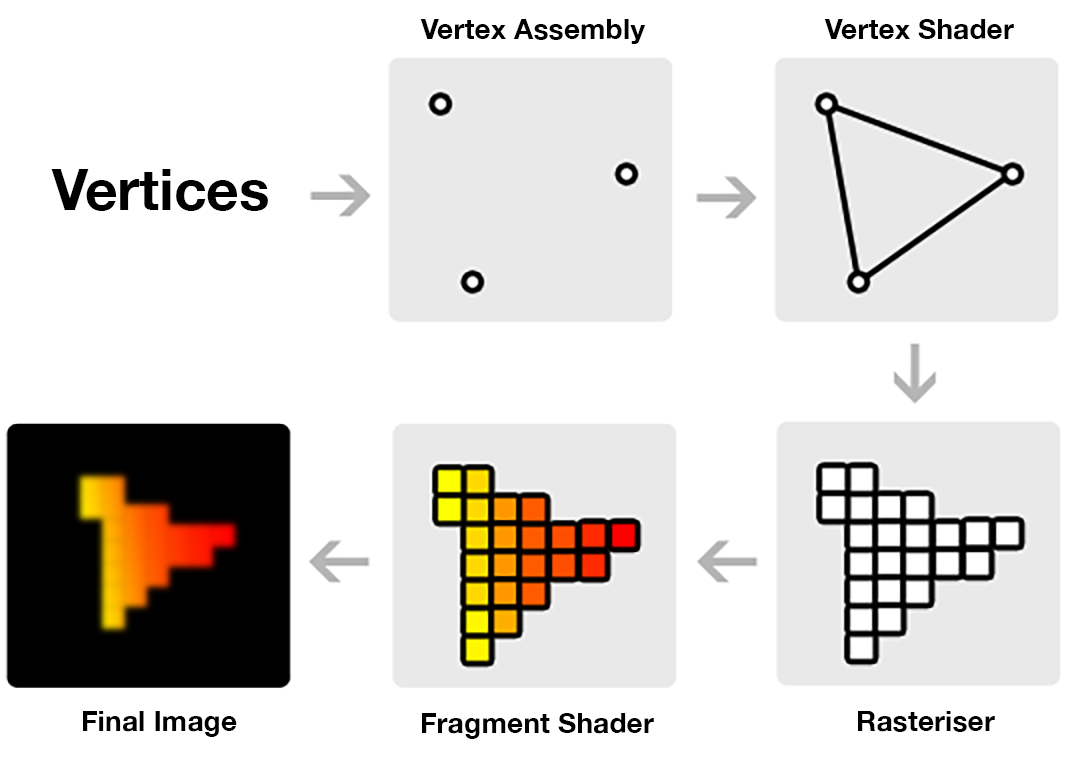
\includegraphics[width=\linewidth]{pipeline}
\caption{A diagram of a basic graphics pipeline, simplified from the original image from \citet{PipelineImage}}
\label{fig:pipeline}
\end{figure}

\textbf{Vertex Input Assembly} is the initial stage, in which data is transferred to the GPU. The majority of this data is the vertices themselves, which are 3D vectors in world-space. These are in sets of three which represent the corners of a triangle, the simplest possible shape that has area; this is the minimum requirement for rendering surfaces (points and lines can be rendered with fewer vertices, but we will only discuss triangles for now).

In addition to world-space vectors, each vertex may have a variety of other data associated with it. This is called \emph{per-vertex data} or \emph{vertex attributes}. Some examples are vertex colours, texture coordinates and pre-computed surface normals. Since this stage represents the boundary between the CPU and GPU, data is transferred in large, contiguous blocks, rather than one vertex or triangle at a time, in order to mitigate the relatively slow communication due to the speed limit of electrons between two computer components that are often multiple inches apart, compared to \emph{e.g.} two cores in one CPU.

A block of per-vertex data may have the corners of triangles laid out in physical memory as xyz xyz xyz xyz xyz xyz xyz..., known as \emph{Structure-of-Arrays}, or xxxx yyyy zzzz xxx yyyy zzzz..., \emph{Array-of-Structures-of-Arrays}. These details need to be communicated to the GPU at this stage. A complete explanation and demonstration of this is given later in the paper, when SIMD is implemented in section \ref{sec:simd}.

Along with the per-vertex data, \emph{modelview} and \emph{projection} matrices for transforming the vertices into \emph{normalised-device-space} are commonly transferred to the GPU. This differs based on whether a \emph{perspective} view or \emph{orthographic} view is desired. However, these transformations are not used in this project; all our coordinates on the CPU are in normalised-device-space as we don't need to transform the view in order to produce a simple orthographic view.

The \textbf{Vertex Shader} is the next stage. It is a customisable program that operates on a single vertex at a time. Like all shaders, many instances of the program are running simultaneously to enable fast throughput. The vertex shader involves the actual transformation from world-space to normalised-device-space; the latter is a three-dimensional coordinate system in which each axis extends from -1 to +1. This space makes the pipeline more efficient as anything outside of this range can be discarded before rasterisation.

Many other operations can be performed in the vertex shader, and an beneficial optimisation process can be to move work from the fragment shader into the vertex shader where possible (\emph{e.g.} per-vertex lighting vs. per-fragment lighting), since there are many more generated fragments than there are vertices, making per-fragment operations more time-consuming. The shader can pass miscellaneous data on to be utilised in later stages.

\textbf{Rasterisation} follows the vertex shader. This is where anything outside of normalised-device-space is discarded. Triangles are converted into \emph{fragments}, which are discrete data in pixel-space. This is done by flattening device-space triangles to 2D creating fragments based on whether the locations of pixels fall within those triangles.

The fragments of triangles that are hidden behind others are discarded here in a process known as \emph{depth-testing}, which involves the use of a depth buffer to record and compare each fragment's depth in the scene, in order to allow triangles to occlude and intersect each other correctly.

The \textbf{Fragment Shader} is the final stage in a simple graphics pipeline. Its main responsibility is to produce the final colour of each pixel. Any per-vertex data that has been passed on by the vertex shader gets transformed into per-fragment data; a vertex attribute that differs for each of the three corners of a triangle will be interpolated based on the position of the fragment in relation to the vertices. This is useful for lots of tasks, including generating per-fragment surface normals efficiently, since there is bespoke hardware on the GPU that performs this task before the fragment shader executes. The per-fragment data can then be observed by the fragment shader and the colour of the final pixel is computed.

% TODO: colour blending, rendering to textures, uniforms. "to be clear, this is just one way to construct a graphics pipeline. "

\subsection{The Vulkan API}

Vulkan is a cross-platform Application Programming Interface for rendering 3D graphics in real-time \citep{Vulkan}. It is developed by the non-profit consortium, the Khronos Group (\citeyear{Khronos}). Along with its contemporaries, Direct3D 12 \citep{d3D12} and Metal \citep{AppleMetal}, it exists to provide graphics programmers with more control over the entire graphics pipeline, enabling a better balance in workload between the CPU and GPU. This was in response to its precursors, namely Direct3D 11 \citep{d3D11} and OpenGL \citep{OpenGLDocs}, which were often bottlenecked by the single-threaded performance of the CPU \citep{CpuBottleneck}.

% TODO: Mention SPIR-V etc?

\subsection{Multi-threading}

Concurrent execution is the very common technique in modern computing of running multiple threads in a single program; the effect is equivalent to two or more processes with access to the same memory. This allows a CPU with multiple cores to run more than one of these threads at once. Amdahl's law or Amdahl's argument \citep{Rodgers1985} shown below is a formula describing the theoretical speedup of a task when the system's resources are improved, such as when more CPU cores are added:

\begin{center}
\begin{Large}
$speedup(s) = \frac{1}{(1-p)+\frac{p}{s}}$
\end{Large}
\end{center}

Where $speedup$ is the overall speed increase of the entire task, $s$ is the speed increase of the part of the task that is improved by better system resources, and $p$ is the original proportion of execution time that the improved part of the task occupied.

Amdahl's law in its most optimistic case is when $p = 1$, which greatly simplifies to $speedup(s) = s$. If we improve the system by adding more processing cores, we introduce $c$, the number of processing cores in the system: $speedup(s) = cs$. Since $c$ is a coefficient of $s$, every increment to $c$ will result in a continually diminishing increase in $speedup(s)$.

This means that a single-threaded task that requires a constant amount CPU time can reach a fraction of that time if rewritten as a multi-threaded task, but every additional core yields diminishing returns (see Figure \ref{fig:cpu_cores}).

\begin{figure}[h]
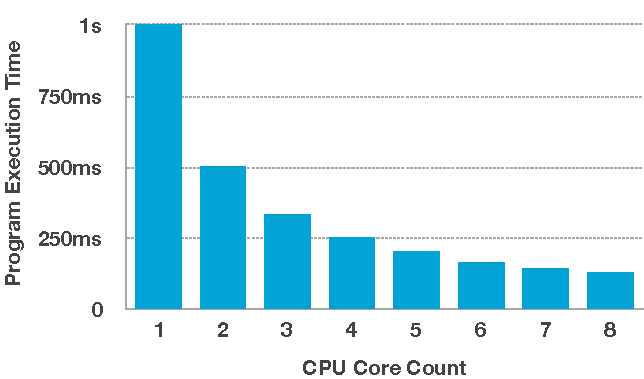
\includegraphics[width=\linewidth]{cpu_cores}
\caption{An example of Amdahl's law \citep{Rodgers1985}: The best-case execution time of a task that requires one second of CPU time, by processor core count.}
\label{fig:cpu_cores}
\end{figure}

\section{Literature Review}

% TODO: \subsection{Performance Profiling}?

\subsection{Particle System Design}

\citet{Tatarchuk2006} has shown many impressive techniques for rendering various effects for a realistic rainy night in a city. Of particular note was skillful use of particles based on pre-blurred normalmaps to create transparent water droplets that have realistic specular highlights from the surrounding streetlights. This is used convincingly both as rain directly from the sky and also as more of a waterfall-like effect to show water gushing out of drainpipes (see Figure \ref{fig:tatarchuk}). The water would then splash into puddles using a pre-rendered splash sequence. The otherwise easy-to-spot repetitiveness of this splash was hidden by randomising the size and transparency of those particles, as well as flipping them horizontally. This could perhaps be improved even further by making larger splashes animate slightly slower, so that the actual simulated falling speed of the droplets within the splash would be convincingly similar regardless of particle size. An additional visual improvement could involve spawning new, tiny droplets in a generally upward velocity at the point of the biggest splashes; this could emphasise the impact of the splash. % TODO: Delve into this paper more?

\begin{figure}[h]
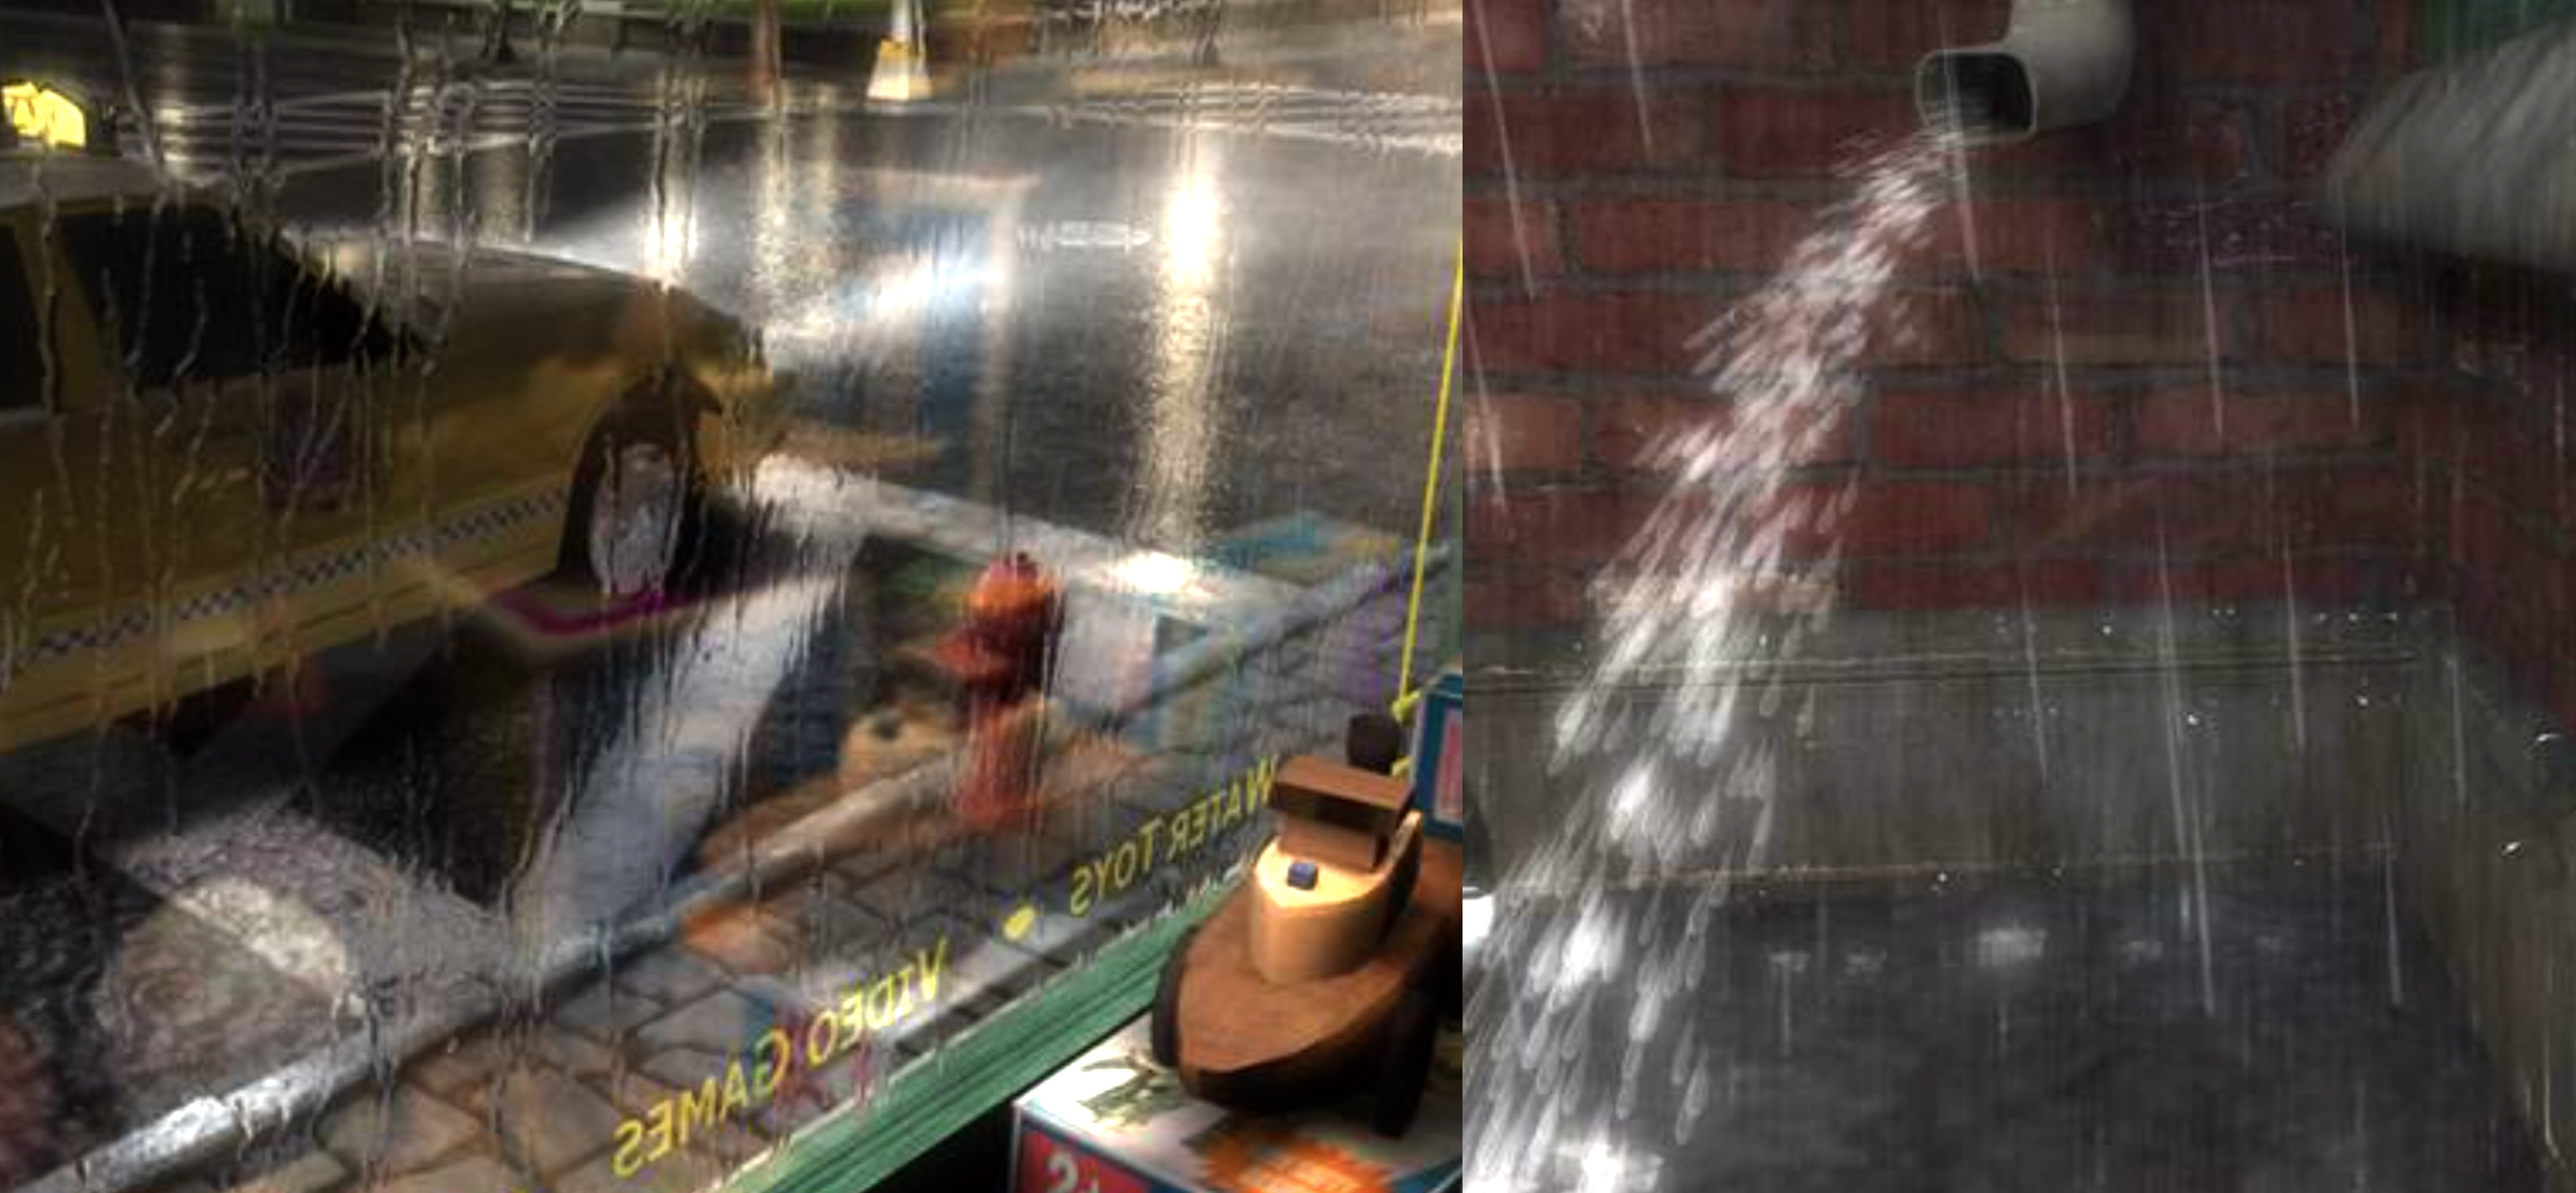
\includegraphics[width=\linewidth]{tatarchuk}
\caption{Work by \citet{Tatarchuk2006} on various rain effects.}
\label{fig:tatarchuk}
\end{figure}

\citet{Boulianne2007} implemented a biological system simulator using a 3D grid in which each element can hold one or zero particles. Their simulator needed to take into account the spacial locality of particles; a grid facilitates this by removing the need for distance calculation and particle search. Although their implementation did not have real-time graphics in mind, this grid-based approach could be applied to particle-based rendering for situations where the intended effect requires particles to react to each other based on their proximity. (TODO: That's called spatial hashing!) Additionally, \citet{Boulianne2007} states ``this system is expected to be suitable for acceleration with parallel customizable hardware,'' meaning this technique would likely be appropriate for rendering real-time particle systems and the parallel nature of GPUs.

\subsection{Techniques for Efficient Real-time Graphics}

\citet{Crawford2018} noted that shader compiler optimisation can make a modest improvement to graphics performance, but it is highly dependent on shader code itself. With their test suite of the LunarGlass/LLVM optimisation framework and the GLSL shaders from GFXBench 4.0, they found that shaders can be sped up by as much as 25\% by finding the best combination of compiler flags, but 1-4\% should be expected in general. Common optimisations that shader compilers can perform are dead code elimination, factoring out conditionals, unrolling loops, coalescing multiple vector element assignments into a single swizzled (TODO: explain swizzling. VkImageViewCreateInfo uses it) vector assignment, global value numbering causing variable elimination, and simplifying arithmetic by reordering the statements. The study reviewed only source-to-source optimisations; source-to-machine-code optimisations weren't explored. Further speed-ups could be found in that area.

Referring to Vulkan and Direct3D 12, \citet{Joseph2016} states ``the central focus of this new generation of APIs is to increase the amount of draw calls possible while decreasing the amount of overhead for the CPU.'' As graphics programmers, we can reinterpret this to indicate that it is critical to reduce the amount of time that the CPU and GPU are required to block each other to communicate, in order to get the most out of the hardware.

\subsection{Multi-threaded Software Design}

Coordination between threads is a necessary characteristic of reliable multi-threaded systems \citep{Powell}. Without coordination, race conditions and simultaneous unsafe memory accesses can occur, leading to unintended, unpredictable behaviour, often resulting in crashes due to memory access violations. Some ways to avoid these issues are presented below.

\textbf{Mutexes} are perhaps the most common mechanism to ensure thread coordination. A thread can attempt to \emph{lock} a mutex; if the mutex was previously in an unlocked state, the attempt to lock is successful and that thread can continue as normal. The thread now "owns" the mutex. If the mutex is already locked, in most cases the thread will be blocked, and will wait until another thread \emph{unlocks} the mutex (only the owning thread can unlock a mutex). The exception to this is when a \verb|try_lock()| function or equivalent is called on the mutex instead of \verb|lock()|; this will not block the thread, and will instead give the opportunity for the thread to do other work while it waits for  Not all mutex implementation have \verb|try_lock()|, but this functionality is available for this project as part of C++'s \verb|std::mutex| \citep{CppMutex}.


% TODO: talk about how I'm using semaphores in Vulkan
\textbf{Semaphores} come in various kinds, but in general they are thread-safe counters. Specifics as to how a semaphore is used is up to its API and the programmer's needs, but a common convention is for a thread to perform a \verb|wait()| operation on a semaphore, which will cause the thread to block until the semaphore's counter is greater than zero. At that point, or if it was already greater than zero, the semaphore will decrement by one and the thread will continue executing. A \verb|post()| can be performed by any thread, which will increment the semaphore. If the counter is above zero and there is at least one thread waiting on the semaphore, one thread can now continue as stated above \citep{BoostSync}.

A semaphore that is always either one or zero is equivalent to a mutex, except for one difference: A \verb|post()| operation can be performed by any thread that has access to the semaphore, allowing any thread to unblock execution, instead of just the thread which called \verb|wait()|.

Semaphores are being introduced into the C++ standard library as part of C++20 \citep{C20Sync}, so they aren't available to our C++17 environment but we could use a separate library for this functionality if necessary, such as the Boost library collection's \verb|interprocess_semaphore|, \verb|named_semaphore|, and \verb|anonymous_semaphore|.

% TODO: Talk in more detail about different kinds of thread blocking like deadlocking.
Blocked threads are a significant cause of the reduction of maximum theoretical performance on multi-core systems \citep{Alemany1992}. In the worst case, a \emph{deadlock} can occur when all threads are blocked, waiting on each other indefinitely. In the case of mutexes, a good rule of thumb is to keep the areas of the program that are mutex-guarded as small, simple and fast as possible, to reduce the amount of time that mutexes are locked, thereby reducing the chance of blocked threads.

Although the effects of thread-blocking can be a significant challenge to remove entirely, there exist programming techniques that allow concurrent sections to communicate without blocking each other, such as \emph{exponential backoff}, an algorithm commonly used in network coordination, that slows a process or thread in order to reduce congestion on a shared resource such as an Ethernet node \citep{Goodman2019}, or more applicably for us, a mutex or critical memory. This of course has the downside of one or more threads not operating at their maximum speed but it can have an overall benefit, depending on the bottlenecks of the program.

\emph{Optimistic concurrency control} is another class of algorithms for non-blocking concurrency that involves validating a transaction performed on shared data before committing it \citep{Herlihy1993} in an attempt to detect whether data corruption had occurred due to simultaneous writes or reads. Again, this has a downside of requiring extra work per transaction.

% "" (some of these techniques) are very complex; their usefulness must be weighed against the development team's ability to handle the additional complexity, and the cost of time spent implementing it. For this reason, we began implementing the optimisation techniques that appeared to have a good benefit-to-complexity ratio. % TODO: make a chart of these ratios?

% good structure from "SunOS Multithread Architecture": The remainder of this paper is divided into N sections. The first section gives an overview of the architecture and introduces our terminology. The second section discusses our design goals and principles. The third section gives additional details of operation and interfaces and how the UNIX process model is reinterpreted in the new environment. The fourth section gives some performance data and operational experience. The last section compares this architecture with others.

\section{Methodology}

A particle system will be built in C++17 and Vulkan 1.1 to resemble spraying water, similar to some of the drainpipe work done by \citet{Tatarchuk2006}. Vertical synchronisation, the option to synchronise the framerate with the vertical refresh rate of the monitor, will be turned off and the program will calculate the duration of the slowest frame out of every one hundred frames (the 99th percentile) and print it to the console.

% TODO: why use 99th?

The amount of particles rendered per frame will be set to 100,000, 200,000, 300,000, 400,000, and 500,000. These numbers will be plotted alongside the frame durations. This will give indications as to whether any optimisation has its greatest effect on high or low particle counts.

The individual functions of the program will be profiled using tools such as Visual Studio's performance analyzer \citep{VSPerfTools} in order to gain an understanding of which parts of the code could be improved. The program will be optimised in stages. At every stage, the performance will be re-examined, new plots will be produced, and the next optimisation steps will be researched and evaluated.

\subsection{Equipment}

We will be designing, profiling and optimising the program for a desktop computer with an Intel Core i5 6400 at 2.7-3.3 GHz with four cores, 8GB of DDR4 RAM at (TODO: what frequency?) and an Nvidia Geforce GTX 1060 3GB. This  graphics card is the most common among Steam users with a 14.5\% share at the time of writing \citep{SteamSurvey}. Valve/Steam's published data on their users' CPUs suggests that at least 25\% of users own a CPU with the same core count and a similar frequency as our i5 6400. 8GB is also the most popular memory amount at 37.1\% of users, so this setup in all should give us a good example of how this program would perform on an average user's system.

% TODO: Note about the CPU not having more threads than cores? (4:4)

% TODO: Talk about how we will profile it. Vulkan layers, Visual Studio's tools etc.

\section{Initial Implementation}

% (Describe the design decisions of the program before any optimisation is performed, and any Vulkan-specific implementation details relevant to the project.)
% My implementation never requires reallocating particles! Brag! It also simplifies SOA so we don't need to do AOSOA!

A Windows application was built in C++17, using version 2.0.10 of the SDL library (\citeyear{SDL2}) for window creation and frame duration calculation. Version 0.9.9.6 of the GLM library (\citeyear{GLM}) was used to provide a 3D vector class along with functionality for vector mathematics.

A particles.cpp file was created that updates an array of \verb|Particle| structures every frame, containing 3D positions and scalar brightness values as shown:

\begin{minted}[fontsize=\footnotesize]{C++}
struct Particle {
  vec3 position;
  float brightness;
};
\end{minted}

Particle velocities were stored in a separate array since they didn't need to be sent to the GPU. Updating the particles functioned by slightly reducing their velocities to simulate air resistance, increasing the downwards velocity to simulate gravity, and applying the velocities to each particle as follows:

\begin{minted}[fontsize=\footnotesize]{C++}
void updateOneParticle(int32_t i, float stepSize) {
  velocities[i] *= 1 - stepSize * airResistance;
  velocities[i].y += gravity * stepSize;
  particles[i].position += velocities[i] * stepSize;

  if (particles[i].position.y > groundLevel) {
    respawn(&particles[i], &velocities[i]);
  }
}

void update(int particleCount, float deltaTime) {
  float stepSize = deltaTime * 0.5f;

  for (int i = 0; i < particles.size(); i++) {
    updateOneParticle(i, stepSize);
  }
}
\end{minted}

Notice the call to \verb|respawn()|. When a particle reaches a ground level \verb|1.0f|, this function is called to reset the particle's position, randomise its brightness, and set its new velocity with a degree of randomness.

This algorithm has the problem of not intelligently spreading out the particles evenly across the scene, but this is not an issue in practice as the particles are positioned at a different height at the beginning of the program, such that they each take a different amount of time to hit ground level. This spreads out the respawn events across time.
% TODO: "this is not a robust way to solve this problem for a real game" etc

A Vulkan 1.1 graphics system was created in graphics.cpp that consumes the array of \verb|Particle| structures and sends them to the GPU. The Vulkan setup code was designed to find a graphics device whose driver supports a single \verb|VkQueue| (a queue for executing GPU-bound commands) that can process both graphical and surface presentation commands. This is done by checking for the \verb|VK_QUEUE_GRAPHICS_BIT| flag and ensuring that \verb|vkGetPhysicalDeviceSurfaceSupportKHR()| returns \verb|true|.
% TODO: diagram or pseudocode describing the vulkan stuff

A vertex shader was written to render one point per particle and adjust the brightnesses based on how close the particle is to the viewer:

\begin{minted}[fontsize=\footnotesize]{C++}
layout(location = 0) in vec3 position;
layout(location = 1) in float brightness;
layout(location = 0) out vec3 outColor;

void main() {
  gl_PointSize = 2;
  gl_Position = vec4(position, 1.0);

  // Set the colour based on brightness and dim the
  // fragment based on the particle's depth (position.z).
  outColor = vec3(brightness, brightness, 1.0);
  outColor *= (0.5 + (position.z-0.5) * 2);
}
\end{minted}

The fragment shader simply coloured the pixels using the value that was passed from the vertex shader:

\begin{minted}[fontsize=\footnotesize]{C++}
layout(location = 0) in vec3 inColor;
layout(location = 0) out vec4 outColor;

void main() {
    outColor = vec4(inColor, 1.0);
}
\end{minted}

\section{Optimisation \& Analysis}

Initial measurements were taken of the program's frame durations. Figure \ref{fig:initialtimes} shows that these times scale mostly linearly by particle count apart from the duration for 500k particles, which showed slightly better proportional performance. However, it was discovered that the 99th percentile of any sample set of frame durations can vary by up to 10\%; the non-linearity of these measurements falls within that margin of error. From this point onwards, efforts were taken to gather typical 99th-percentile measurements that did not appear to be anomalous.
% TODO: Why does the measurement vary? "99th-percentile excacerbates it too"

\begin{figure}[h]
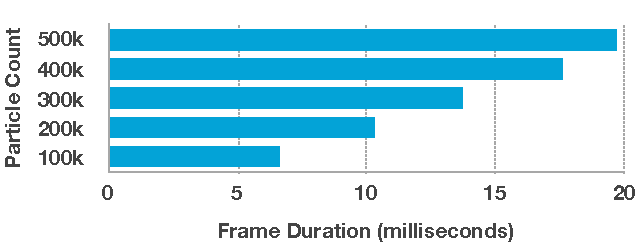
\includegraphics[width=\linewidth]{initialtimes}
\caption{99th-percentile frame durations for different particle counts, before any optimisations were performed.}
\label{fig:initialtimes}
\end{figure}

\subsection{Multithreading \& Random Number Generation}

Profiling the program showed that the function that was taking the most time was \verb|updateOneParticle()| in particles.cpp, but its contents was quite minimal:

\begin{minted}[fontsize=\footnotesize]{C++}
void updateOneParticle(int32_t i, float stepSize) {
  velocities[i] *= 1 - airResistance * stepSize;
  velocities[i].y += gravity * stepSize;
  particles[i].position += velocities[i] * stepSize;

  if (particles[i].position.y > groundLevel) {
    respawn(&particles[i], &velocities[i]);
  }
}
\end{minted}

Notes were made to precalculate \verb|1| \verb|-| \verb|airResistance| \verb|*| \verb|stepSize| and \verb|gravity| \verb|*| \verb|stepSize| in advance so it didn't have to be re-calculated for every call to this function, but at this stage it appeared that parallelising \verb|updateOneParticle()| across all four CPU cores would provide a more significant performance increase. The first attempt at this involved spawning four threads at the start of \verb|update()|. Each thread would repeatedly request new particles to update:

\begin{minted}[fontsize=\footnotesize]{C++}
int32_t requestParticleIndex() {
  int32_t index;
  particleMutex.lock();
  
  if (nextParticleIndexToUpdate < particles.size()) {
  index = nextParticleIndexToUpdate++;
  } else index = -1;
  
  particleMutex.unlock();
  return index;
}
\end{minted}
\begin{minted}[fontsize=\footnotesize]{C++}
void updaterThread(float stepSize) {
  while (true) {
    int32_t i = requestParticleIndex();
    if (i < 0) break;
    updateOneParticle(i, stepSize);
  }
}
\end{minted}

The function that spawned the threads would wait for them to finish by calling their \verb|std::thread::join()| method before returning. After these changes a bug was discovered that caused particles to respawn with poor randomisation of velocities and brightnesses (Figure \ref{fig:randombug}).

\begin{figure}[h]
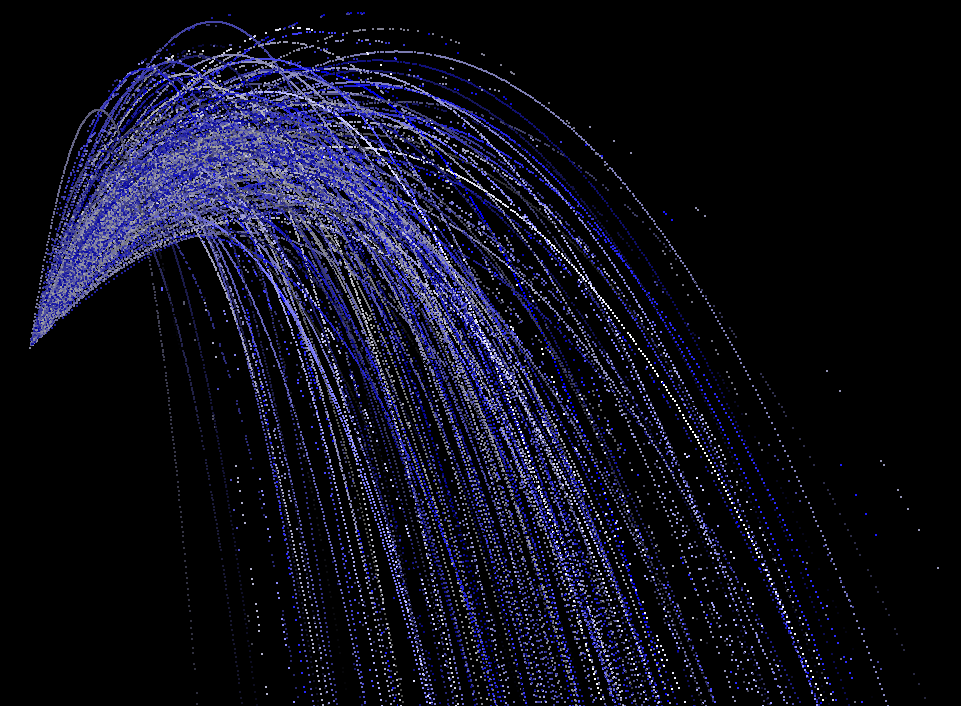
\includegraphics[width=\linewidth]{randombug}
\caption{Unnatural distributions of particles were exhibited after the first multithreading attempt.}
\label{fig:randombug}
\end{figure}

Debugging the program showed that the new multithreading code was performing as expected, so attention was given to the library function being used for random number generation (RNG), \verb|rand()| and \verb|srand()|. To deduce whether the seed generation by \verb|srand()| was thread-local and therefore generating bad values when a seed wasn't given for each thread, experimental code was written that would re-call \verb|srand()| at the start of each thread instead of just once at the start of the program.
% TODO oh hey rand() isn't thread-safe.
% TODO
% TODO
% TODO
% TODO
% TODO
% TODO
% TODO
% TODO
% TODO

\begin{figure}[h]
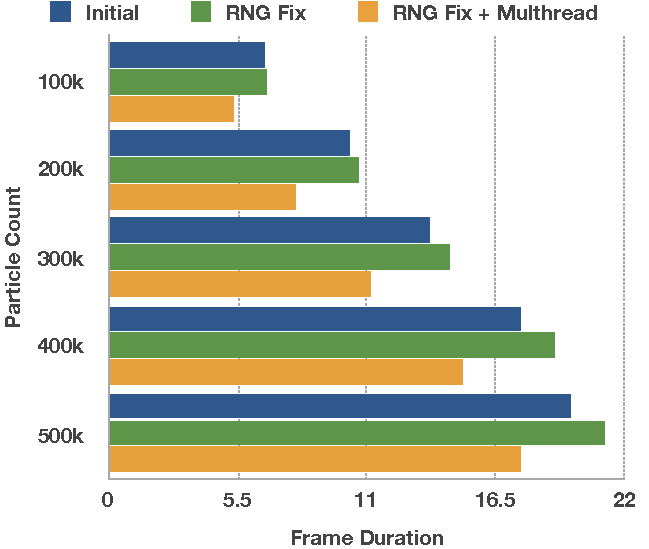
\includegraphics[width=\linewidth]{initial-rng-multithread}
\caption{(placeholder caption)}
\label{fig:initial-rng-multithread}
\end{figure}

\subsection{,mutexless multithread, non-blocking-ish}

\lipsum[1-1]

\begin{figure}[h]
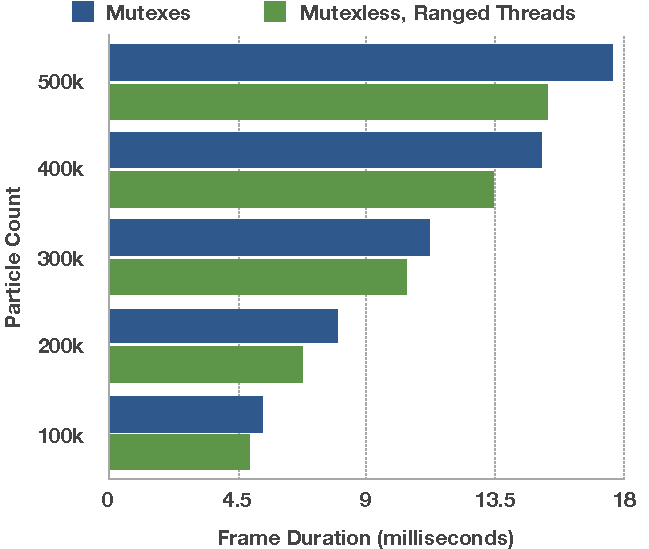
\includegraphics[width=\linewidth]{mutexes-rangedthreads}
\caption{(placeholder capfftion)}
\label{fig:mutexes-rangedthreads}
\end{figure}

\subsection{,const ref}

\lipsum[1-1]

\begin{figure}[h]
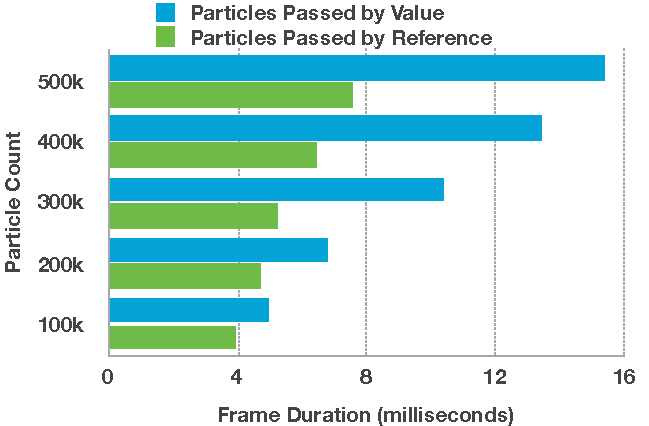
\includegraphics[width=\linewidth]{pass-by-value-reference}
\caption{(placeholder caption)}
\label{fig:pass-by-value-reference}
\end{figure}

\subsection{,no thread recreation}

\lipsum[1-1]

\begin{minted}[fontsize=\footnotesize]{javascript}
Semaphore onUpdateStart;
Semaphore onUpdateComplete;

function initialise() {
  for i in updaterThreadCount {
    spawnThread(updaterThread);
  }
}

function updaterThread() {
  while true {
    onUpdateStart.wait();
    updateParticleRange();
    onUpdateComplete.post();
  }
}

function updateAllParticles() {
  onUpdateStart.post(updaterThreadCount);
  onUpdateComplete.wait(updaterThreadCount);
}
\end{minted}

(((Pseudo-code that updates particles in parallel without recreating threads, synchronised using dual semaphores.))) shows how this is implemented: When \verb|updateAllParticles()| is called on the main thread, it will wait and the \verb|updaterThread|s will each update their own particle ranges. When they are all done, they will notify \verb|updateAllParticles()| on the main thread, which will return. The \verb|updaterThread|s will wait for the next update at the top of their \verb|while| loops, and the main thread is then free to render the newly-updated particles.

\begin{figure}[h]
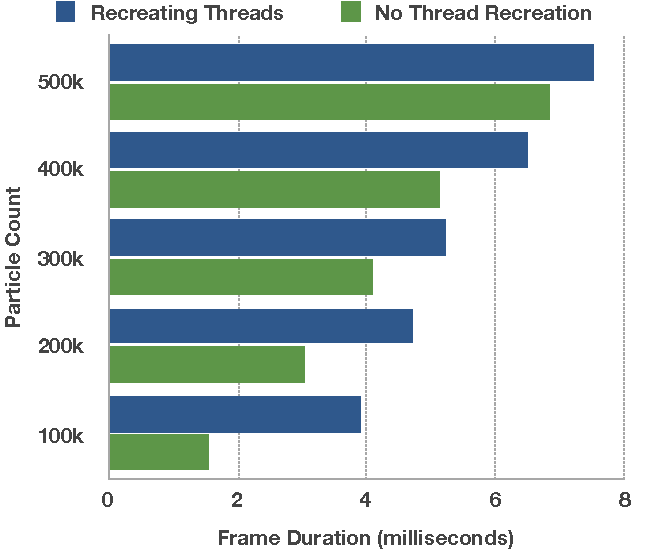
\includegraphics[width=\linewidth]{recreate-no-recreation}
\caption{(placeholder caption)}
\label{fig:recreate-no-recreation}
\end{figure}

\subsection{,simd w conversion} \label{sec:simd}

\lipsum[1-1]

\begin{figure}[h]
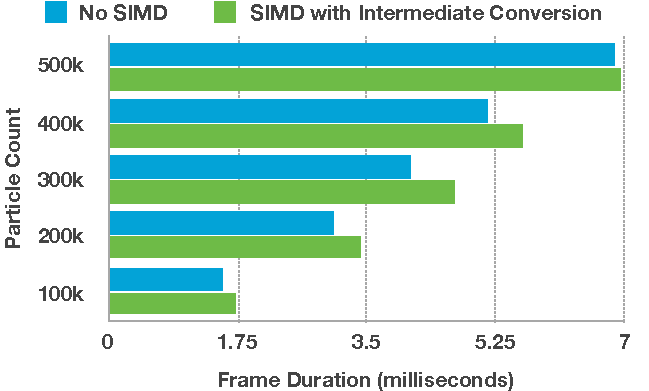
\includegraphics[width=\linewidth]{nosimd-slowsimd}
\caption{(placeholder caption)}
\label{fig:nosimd-slowsimd}
\end{figure}

,the corners of triangles are often stored in CPU-bound memory in an \emph{interleaved} layout as XYZXYZXYZ..., similar to a common left-right layout for audio samples, LRLRLRLR. But sometimes other memory layouts are used, such as XXXYYYZZZ.

\subsection{,simd w direct gpu transfer}

\lipsum[1-1]

\begin{figure}[h]
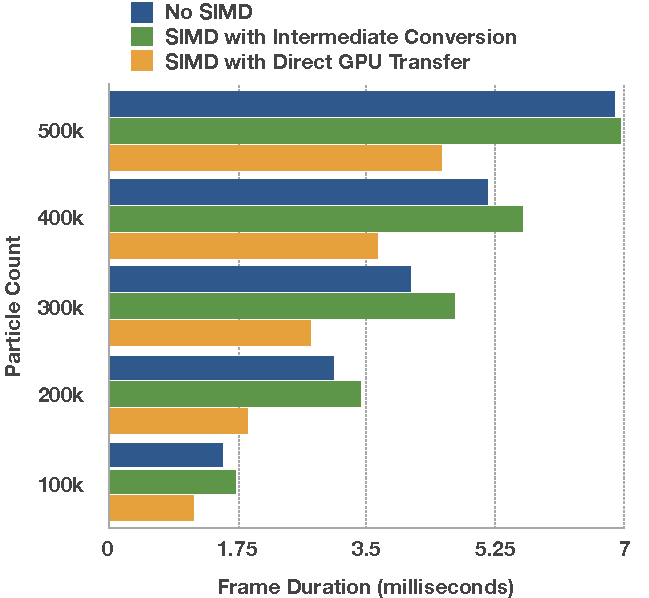
\includegraphics[width=\linewidth]{nosimd-simdwic-simdwdirect}
\caption{(placeholder caption)}
\label{fig:nosimd-simdwic-simdwdirect}
\end{figure}

% (Describe in detail all the optimisation techniques I implemented and the changes in the performance characteristics of the program as I make changes to the code. Describe the critical thought processes along the way. Describe the complexity and other difficulties of implementing each optimisation. Towards the end of this section, focus on analysis including comparisons of related optimisations performed. Include charts showing how performance scales with the amount of particles. Include diagrams showing data pipelines.)

% "At this point" depth testing was implemented. This highlighted that the existing code for updating particles was based on the assumption that particles should move closer to the screen by increasing their position.z variable. However, a convention in depth testing of "lower values mean closer to the screen, and therefore less depth" is more intuitive, so changes were made to the particle system and the vertex shader to flip the usage of the Z axis. Implementing depth-testing and flipping the Z axis did not result in a noticeable change in performance.

\subsection{speedup pies}

\lipsum[1-1]

\begin{figure}[h]
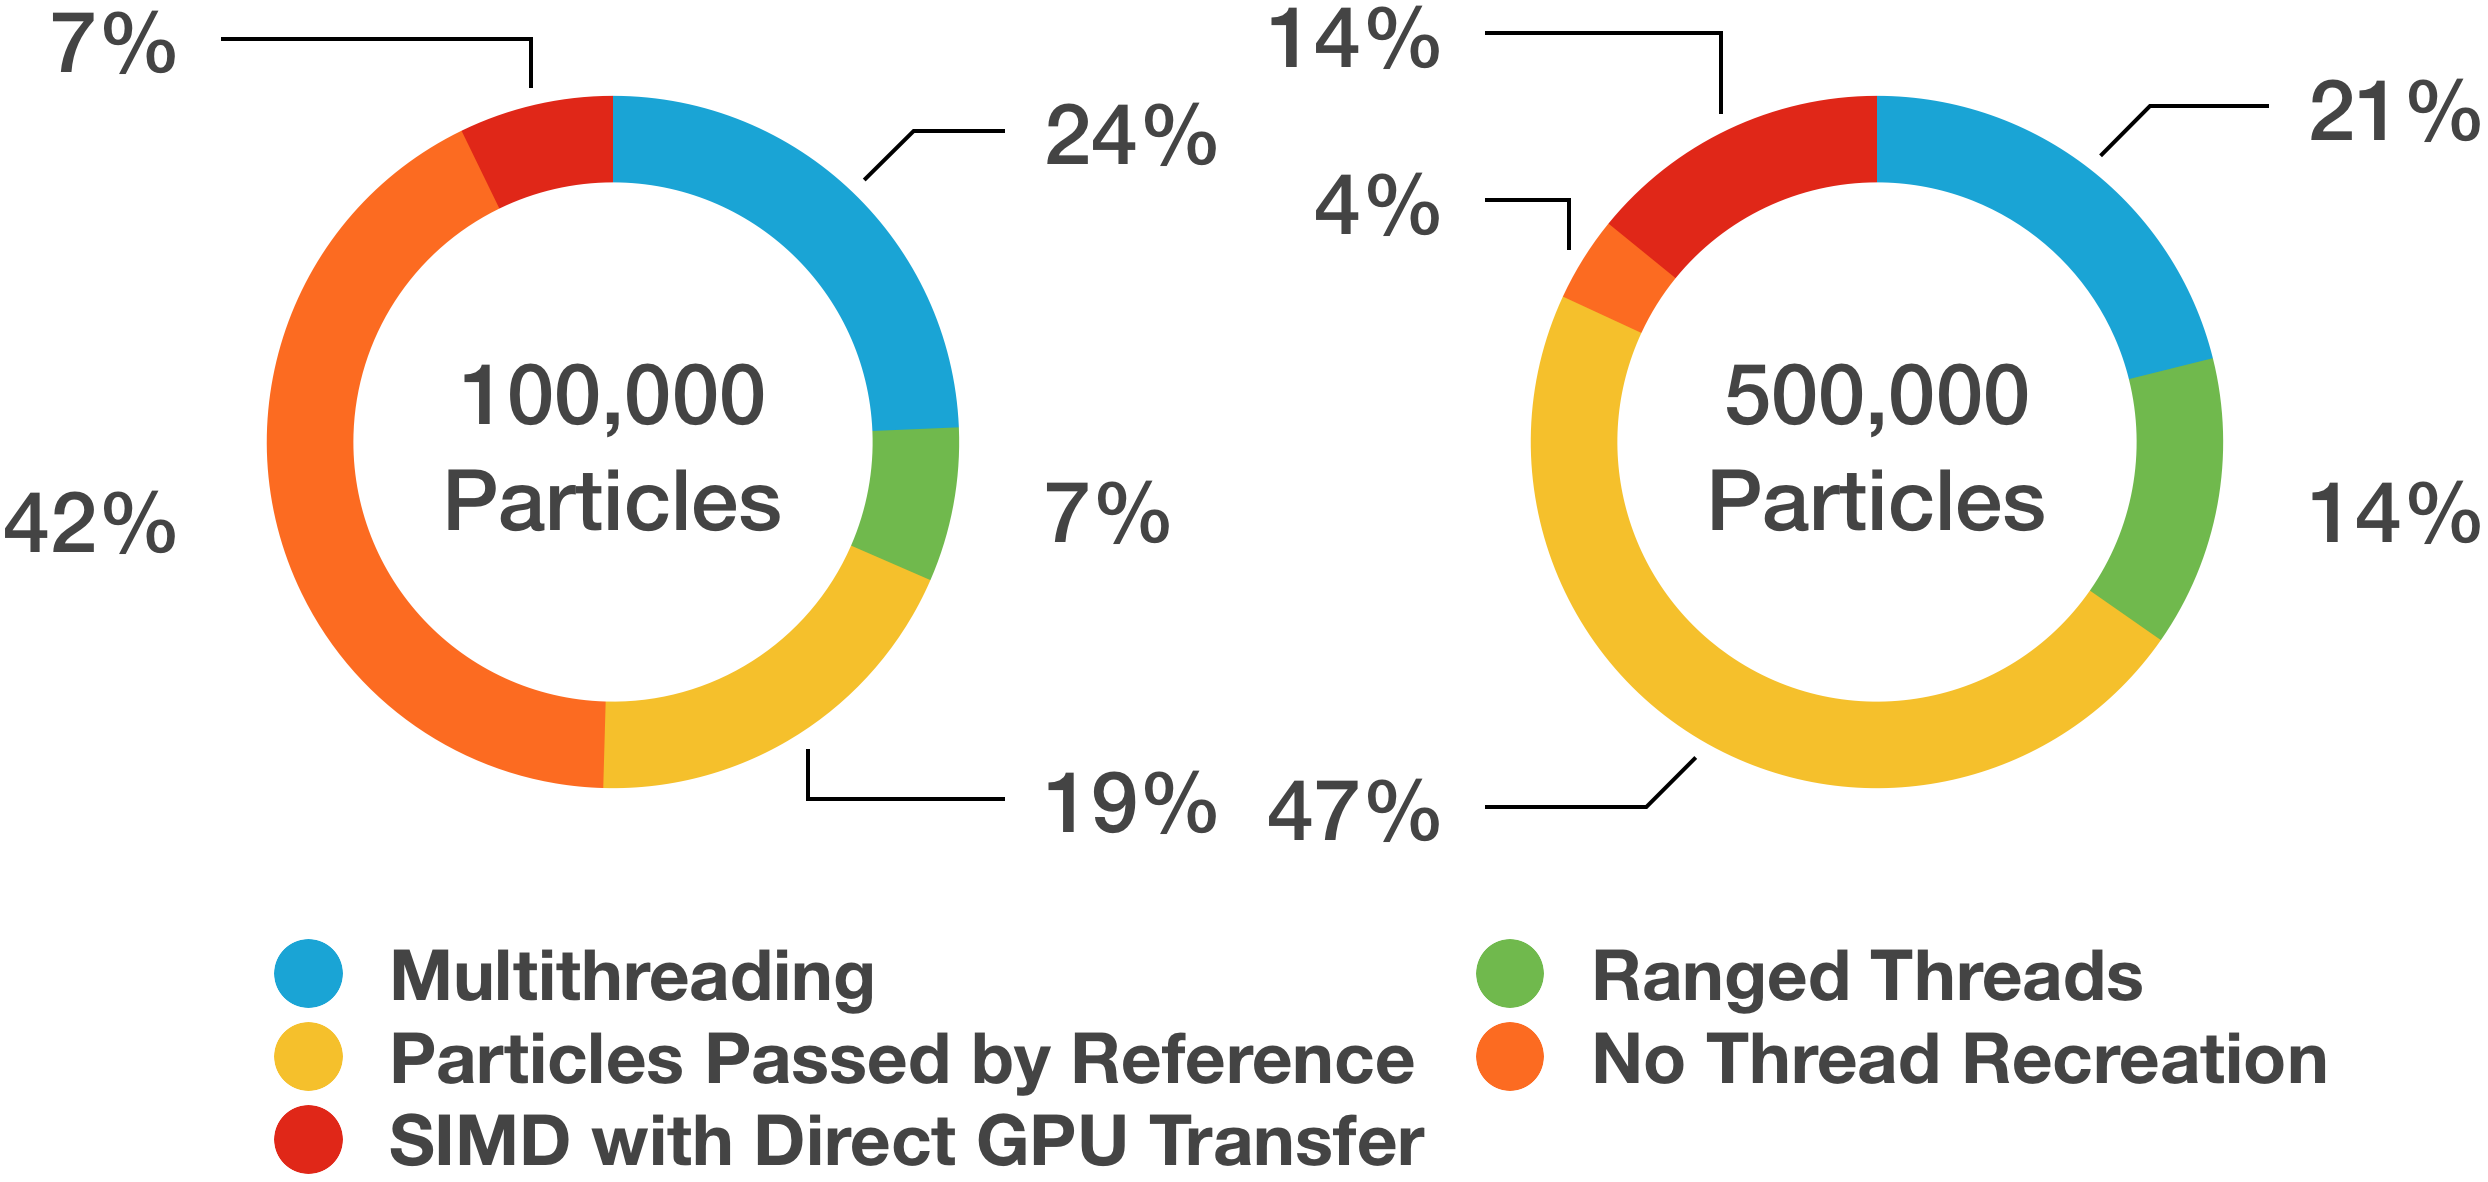
\includegraphics[width=\linewidth]{speedup-pies}
\caption{(placeholder caption)}
\label{fig:speedup-pies}
\end{figure}

\section{Conclusion}

% (Continue to analyse as in the previous section but take a bigger-picture approach and summarise the overall findings. Write in a specific style knowing that some readers will have read the abstract and then jumped to this section.)


%%%%%%%%%%%%%%%%%%%%%%%%%%%%%%%%%%%%%%%%%%%%%%%%%%%%%%%%%%%%%%%%%%%%%%%%%%%%%%%%
\bibliographystyle{agsm}
\bibliography{mendeley_refs, other_refs}

% TODO: appendix entry with full details of the computer - include the protocol and theoretical speed of the GPU's bus etc.
% TODO: appendix entry with notes on Vulkan on macOS with MoltenVK

\end{document}





